\documentclass[11pt]{article}
\usepackage[T1]{fontenc}
\usepackage[utf8]{inputenc}
\usepackage{lmodern}
\usepackage{amsmath,amssymb,amsthm,mathtools,mathrsfs}
\usepackage{enumitem}
\usepackage{graphicx}
\usepackage{microtype}
\usepackage[margin=1in]{geometry}
\usepackage[colorlinks=true,linkcolor=blue,citecolor=blue,urlcolor=blue]{hyperref}

\newtheorem{theorem}{Theorem}
\newtheorem{lemma}[theorem]{Lemma}
\newtheorem{corollary}[theorem]{Corollary}
\newcommand{\D}{\mathbb D}
\newcommand{\N}{\mathbb N}
\newcommand{\T}{\mathbb T}
\newcommand{\Hinf}{\mathcal H^\infty}
\newcommand{\Minf}{\mathcal M_\infty}
\newcommand{\F}{\mathscr F}

\title{Large vector-valued fibers over arbitrary target balls\\
\large A candidate partial answer for arXiv:1902.01387}
\author{Autonomous proof attempt, lane 6}
\date{13 August 2026}

\begin{document}
\maketitle

\begin{center}
\fbox{\parbox{0.90\textwidth}{\textbf{Status: candidate partial result, likely valid.}
The result answers the source question for $X=c_0$ and arbitrary Banach target
space $Y$, and for a corresponding family of fibers when $X$ contains a
1-complemented isometric copy of $c_0$.  It does not settle the question for a
general infinite-dimensional source space $X$.}}
\end{center}

\section{Source question}

For Banach spaces $X,Y$, let $\Minf(B_X,B_Y)$ be the nonzero algebra
homomorphisms from $\Hinf(B_X)$ to $\Hinf(B_Y)$.  The canonical projection
\[
 \xi:\Minf(B_X,B_Y)\longrightarrow
 \overline B_{\Hinf(B_Y,X^{**})}
\]
gives the fiber $\F(g)=\xi^{-1}(g)$.  Dimant and Singer ask whether, for
infinite-dimensional $X$, the fibers over nonconstant maps
\[
 g\in \overline B_{\Hinf(B_Y,X^{**})},\qquad
 g(B_Y)\subset B_{X^{**}},
\]
are large.  They emphasize the unresolved norm-one case: can their analytic
disk theorem be extended to $\|g\|=1$ while every value $g(y)$ remains in the
open ball?  See page 15 of the source PDF and Figure~\ref{fig:question}
\cite{DimantSingerFibered}.

\begin{figure}[ht]
  \centering
  
\includegraphics[width=0.94\textwidth]{figures/open_problem_crop.png}
  \caption{The source question on PDF page 15 of arXiv:1902.01387.}
  \label{fig:question}
\end{figure}

A later paper proves that every fiber of
$\Minf(B_{c_0},B_{c_0})$ contains $2^{\mathfrak c}$ disjoint analytic
Gleason-isometric copies of
$B_{\Hinf(B_{c_0},\ell_\infty)}$ \cite[Theorem 2.4]{DimantSingerPolydisk}.
The target domain in that theorem is again $c_0$.  The first result below
removes that restriction completely.

\section{Proof intuition}

The proof of the later $c_0$ theorem needs a common subsequence of the
coordinate functions $g_n$.  Its published selection lemma invokes a
compactness theorem for bounded holomorphic functions on $B_{c_0}$, which is
the only step apparently tied to the target domain $Y=c_0$.

The replacement is one-dimensional.  Select a subsequence for which the
single scalar sequence $g_n(0)$ converges.  If its limit lies inside the disk,
Schwarz--Pick bounds every selected coordinate uniformly below one at each
fixed $y\in B_Y$.  If the limit lies on the circle, the same inequality forces
pointwise convergence to that unimodular limit throughout $B_Y$.  This is
exactly the dichotomy needed by the original construction, for every Banach
space $Y$.  No compactness or separability of $Y$ is required.

Finally, if $c_0$ is 1-complemented in a source space $X$, restriction from
$B_X$ to that copy of $B_{c_0}$ is a norm-one quotient on the holomorphic
algebras and has a norm-one right inverse.  Precomposing homomorphisms with
this restriction preserves the fiber, analyticity, and the Gleason metric.

\section{The coordinate dichotomy}

Write
\[
 \rho(a,b)=\left|\frac{a-b}{1-\overline b a}\right|
 \qquad(a,b\in\D)
\]
for the pseudo-hyperbolic metric.

\begin{lemma}[target-domain-free coordinate dichotomy]\label{lem:dichotomy}
Let $Y$ be any complex Banach space and let
$(u_n)\subset\overline B_{\Hinf(B_Y)}$.  There is a subsequence
$(u_{n_k})$ for which one of the following holds:
\begin{enumerate}[label=\textup{(\roman*)}]
\item for every $y\in B_Y$,
      $\sup_k |u_{n_k}(y)|<1$;
\item there is $\lambda\in\T$ such that
      $u_{n_k}(y)\to\lambda$ for every $y\in B_Y$.
\end{enumerate}
\end{lemma}

\begin{proof}
Pass to a subsequence, still denoted $(u_n)$, such that
$u_n(0)\to\lambda\in\overline\D$.

Suppose first that $|\lambda|<1$.  Choose $q$ with
$|\lambda|<q<1$ and discard finitely many terms so that
$|u_n(0)|\le q$.  Schwarz--Pick for the holomorphic map
$u_n:B_Y\to\D$ gives
\[
 \rho\bigl(u_n(y),u_n(0)\bigr)\le \|y\|.
\]
Consequently, with $r=\|y\|<1$,
\[
 |u_n(y)|\le \frac{q+r}{1+qr}<1
\]
for every selected $n$.  This proves (i).

Suppose now that $|\lambda|=1$.  For fixed $y\in B_Y$, the same
Schwarz--Pick inequality keeps $u_n(y)$ within pseudo-hyperbolic distance
$\|y\|<1$ of $u_n(0)$.  A sequence in $\D$ at a fixed pseudo-hyperbolic
distance strictly below one from a sequence converging to
$\lambda\in\T$ must itself converge to $\lambda$: after passing to a cluster
point $a\in\overline\D$, the limiting inequality would be
$|a-\lambda|\le r|1-\overline\lambda a|$; the two absolute values are equal
when $|\lambda|=1$, so $r<1$ forces $a=\lambda$.  Thus
$u_n(y)\to\lambda$ for every $y$, proving (ii).
\end{proof}

\section{Main partial theorem}

We use the notation and Gleason metric of
\cite{DimantSingerFibered,DimantSingerPolydisk}.  In particular,
$\F_Y(g)$ denotes the fiber in $\Minf(B_{c_0},B_Y)$.

\begin{theorem}[arbitrary target domain]\label{thm:arbitraryY}
Let $Y$ be any complex Banach space.  For every
\[
 g\in\overline B_{\Hinf(B_Y,\ell_\infty)}
\]
there is a map
\[
 \Psi_g:(\beta\N\setminus\N)\times
 B_{\Hinf(B_Y,\ell_\infty)}\longrightarrow \F_Y(g)
\]
such that:
\begin{enumerate}[label=\textup{(\arabic*)}]
\item for every $\eta\in\beta\N\setminus\N$, the map
      $\Psi_g^\eta(h)=\Psi_g(\eta,h)$ is an analytic Gleason isometry;
\item if $\eta_1\ne\eta_2$, the images of $\Psi_g^{\eta_1}$ and
      $\Psi_g^{\eta_2}$ lie in different Gleason parts.
\end{enumerate}
In particular, every fiber contains $2^{\mathfrak c}$ pairwise disjoint
analytic copies of the full ball $B_{\Hinf(B_Y,\ell_\infty)}$.
\end{theorem}

\begin{proof}
Write $g=(g_n)_n$, with
$g_n\in\overline B_{\Hinf(B_Y)}$.  Apply
Lemma~\ref{lem:dichotomy}.  This supplies precisely the two alternatives of
\cite[Lemma 2.2]{DimantSingerPolydisk}, now on $B_Y$:
either some coordinate subsequence $g'=(g_{n_k})_k$ satisfies
$g'(B_Y)\subset B_{\ell_\infty}$, or a coordinate subsequence converges
pointwise to a number $\lambda\in\T$.

We spell out why the remainder of the proof of
\cite[Theorem 2.4]{DimantSingerPolydisk} is independent of the target domain.
Let $\mathbb J=\{n_k:k\in\N\}$.  The scalar construction in
\cite[Theorem 1.1 and its proof]{DimantSingerPolydisk} provides maps
$\Phi^k_{z,\mathbb J}(w)$ in the scalar spectrum of $\Hinf(B_{c_0})$.
In the first alternative define, for
$h\in B_{\Hinf(B_Y,\ell_\infty)}$,
\[
 \Psi_g^k(h)(f)(y)
   =\Phi^k_{g(y),\mathbb J}\bigl(h(y)\bigr)(f),
 \qquad f\in\Hinf(B_{c_0}),\ y\in B_Y.
\]
For fixed $k,h,f$, the two-variable map obtained by putting $g(y)$ and
$h(y')$ in the scalar formula is separately holomorphic on
$B_Y\times B_Y$; Hartogs' theorem and restriction to the diagonal show that
$\Psi_g^k(h)(f)$ is holomorphic.  The scalar construction bounds it by
$\|f\|$, so it belongs to $\Hinf(B_Y)$.

The general weak-star compactness of $\Minf(B_{c_0},B_Y)$, established via
the canonical predual $\mathcal G^\infty(B_Y)$ in
\cite[Section 2]{DimantSingerFibered}, lets $k\mapsto\Psi_g^k(h)$ extend to
$\beta\N$.  For $\eta\in\beta\N\setminus\N$ the scalar evaluation identity
is
\[
 \delta_y\circ\Psi_g^\eta(h)
   =\Phi^\eta_{g(y),\mathbb J}\bigl(h(y)\bigr).
 \tag{1}
\]
It gives $\xi(\Psi_g^\eta(h))=g$.  The scalar maps are Gleason isometries,
so taking the supremum of their pseudo-hyperbolic equalities over
$y\in B_Y$ proves that $\Psi_g^\eta$ is a Gleason isometry.  Distinct
ultrafilters give scalar images in different Gleason parts; (1) transfers
this separation to the vector-valued spectrum.  Analyticity in $h$ follows
pointwise from the analytic scalar maps and then from the general
point-evaluation criterion for locally bounded maps into $\Hinf(B_Y)$
\cite[Lemma 2.3]{DimantSingerFibered}.

In the second dichotomy alternative, if $\lambda\ne1$, then for every fixed
$y$ the selected coordinates $g_{n_k}(y)$ are eventually a positive distance
from $1$.  This is exactly the second case of the proof of
\cite[Theorem 2.4]{DimantSingerPolydisk}, and the preceding construction
applies.  If $\lambda=1$, multiply the selected coordinates by a fixed
unimodular scalar different from $1$ and use the coordinate-rotation Gleason
isometry of \cite[Lemma 2.3]{DimantSingerPolydisk}.  These operations concern
only the $c_0$ source coordinates and are unchanged when $B_{c_0}$ in the
target variable is replaced by $B_Y$.  This proves both assertions.
\end{proof}

\begin{corollary}[the $c_0$ case of the source question]\label{cor:c0}
For every Banach space $Y$, every nonconstant
$g\in\overline B_{\Hinf(B_Y,\ell_\infty)}$ satisfying
$g(B_Y)\subset B_{\ell_\infty}$ has a large fiber in the strongest sense of
Theorem~\ref{thm:arbitraryY}.  This includes all such maps with $\|g\|=1$.
\end{corollary}

\begin{proof}
Apply Theorem~\ref{thm:arbitraryY}; its conclusion holds for every $g$ in the
closed ball, without requiring either nonconstancy or pointwise interiority.
\end{proof}

\section{Transfer through a complemented copy of \texorpdfstring{$c_0$}{c0}}

\begin{theorem}[complemented-$c_0$ transfer]\label{thm:transfer}
Let $X,Y$ be complex Banach spaces.  Suppose there are norm-one maps
\[
 J:c_0\longrightarrow X,\qquad P:X\longrightarrow c_0,\qquad PJ=I_{c_0},
\]
with $J$ an isometry.  For every
$g_0\in\overline B_{\Hinf(B_Y,\ell_\infty)}$, the fiber in
$\Minf(B_X,B_Y)$ over $J^{**}\circ g_0$ contains the images furnished by
Theorem~\ref{thm:arbitraryY}, with analyticity and all Gleason distances
preserved.  Hence it contains $2^{\mathfrak c}$ disjoint analytic
Gleason-isometric copies of $B_{\Hinf(B_Y,\ell_\infty)}$.
\end{theorem}

\begin{proof}
Define
\[
 R:\Hinf(B_X)\to\Hinf(B_{c_0}),\quad Rf=f\circ J,
 \qquad
 E:\Hinf(B_{c_0})\to\Hinf(B_X),\quad Eu=u\circ P.
\]
Both are norm-one unital algebra homomorphisms, $RE=I$, and $E$ is an
isometry.  For
$\Theta\in\Minf(B_{c_0},B_Y)$ put
\[
 L\Theta=\Theta\circ R\in\Minf(B_X,B_Y).
\]
If $\Theta\in\F_Y(g_0)$ and $x^*\in X^*$, then
\[
 (L\Theta)(x^*)(y)
 =\Theta(J^*x^*)(y)
 =g_0(y)(J^*x^*)
 =(J^{**}g_0(y))(x^*).
\]
Thus $L\Theta$ lies in the fiber over $J^{**}\circ g_0$.

The equality $RE=I$ makes $L$ injective.  More precisely, for scalar
characters $\varphi,\psi$ on $\Hinf(B_{c_0})$, the unit ball under $R$ is
exactly the unit ball of $\Hinf(B_{c_0})$: one inclusion follows from
$\|R\|=1$, and the reverse inclusion follows by applying $E$.  Therefore
\[
 \rho(\varphi\circ R,\psi\circ R)=\rho(\varphi,\psi).
\]
Taking the supremum over $y\in B_Y$ shows that $L$ preserves the
vector-valued Gleason metric.  Since $L$ is bounded linear on the ambient
operator spaces, it also preserves analyticity.  Apply $L$ to all the copies
from Theorem~\ref{thm:arbitraryY}.
\end{proof}

\section{Verification, scope, and novelty status}

The new mathematical input is Lemma~\ref{lem:dichotomy}; every inequality in
it is scalar Schwarz--Pick.  Theorem~\ref{thm:arbitraryY} then audits the
published proof step by step: scalar $c_0$-fiber maps, Hartogs, weak-star
compactness, the evaluation identity, and the point-evaluation holomorphy
criterion are all stated for general Banach target domains or depend only on
the $c_0$ source.  Theorem~\ref{thm:transfer} is an exact algebraic
restriction/right-inverse argument.

This is only a partial answer to arXiv:1902.01387.  It does not construct
coherent analytic families in scalar fibers for a general infinite-dimensional
$X$.  The known fact that each individual scalar fiber is large supplies no
such dependence on $g(y)$, and the source proof's strict-ball perturbation loses
all uniform radius when $\|g\|=1$.

A bounded novelty check searched the run indexes and arXiv for the source id,
the later $c_0$ paper, ``vector-valued spectrum'', ``$c_0$'', arbitrary or
separable Banach target spaces, and large fibers.  It found the exact
$X=Y=c_0$ theorem in arXiv:1909.05105 and the distinct uniform-algebra Hilbert
space paper arXiv:2102.06771, but no statement extending Theorem 2.4 to
arbitrary $Y$ or transferring it through a complemented $c_0$.  This is a
bounded search, not a definitive novelty certification.

\paragraph{Human-review recommendation.}
Review as a likely valid partial result.  The highest-value checks are that
the scalar construction used in the two cases of
\cite[Theorem 2.4]{DimantSingerPolydisk} has no hidden dependence on the target
domain, and that its weak-star ultrafilter limit remains exactly the general
$\Minf(B_{c_0},B_Y)$ compactness described in
\cite{DimantSingerFibered}.

\clearpage
\section*{Supporting theorem evidence}
Figures~\ref{fig:support9} and \ref{fig:support10} reproduce PDF pages 9--10
of arXiv:1909.05105, containing Lemmas 2.2--2.3, Theorem 2.4, and the part of
its proof generalized above.

\begin{figure}[ht]
  \centering
  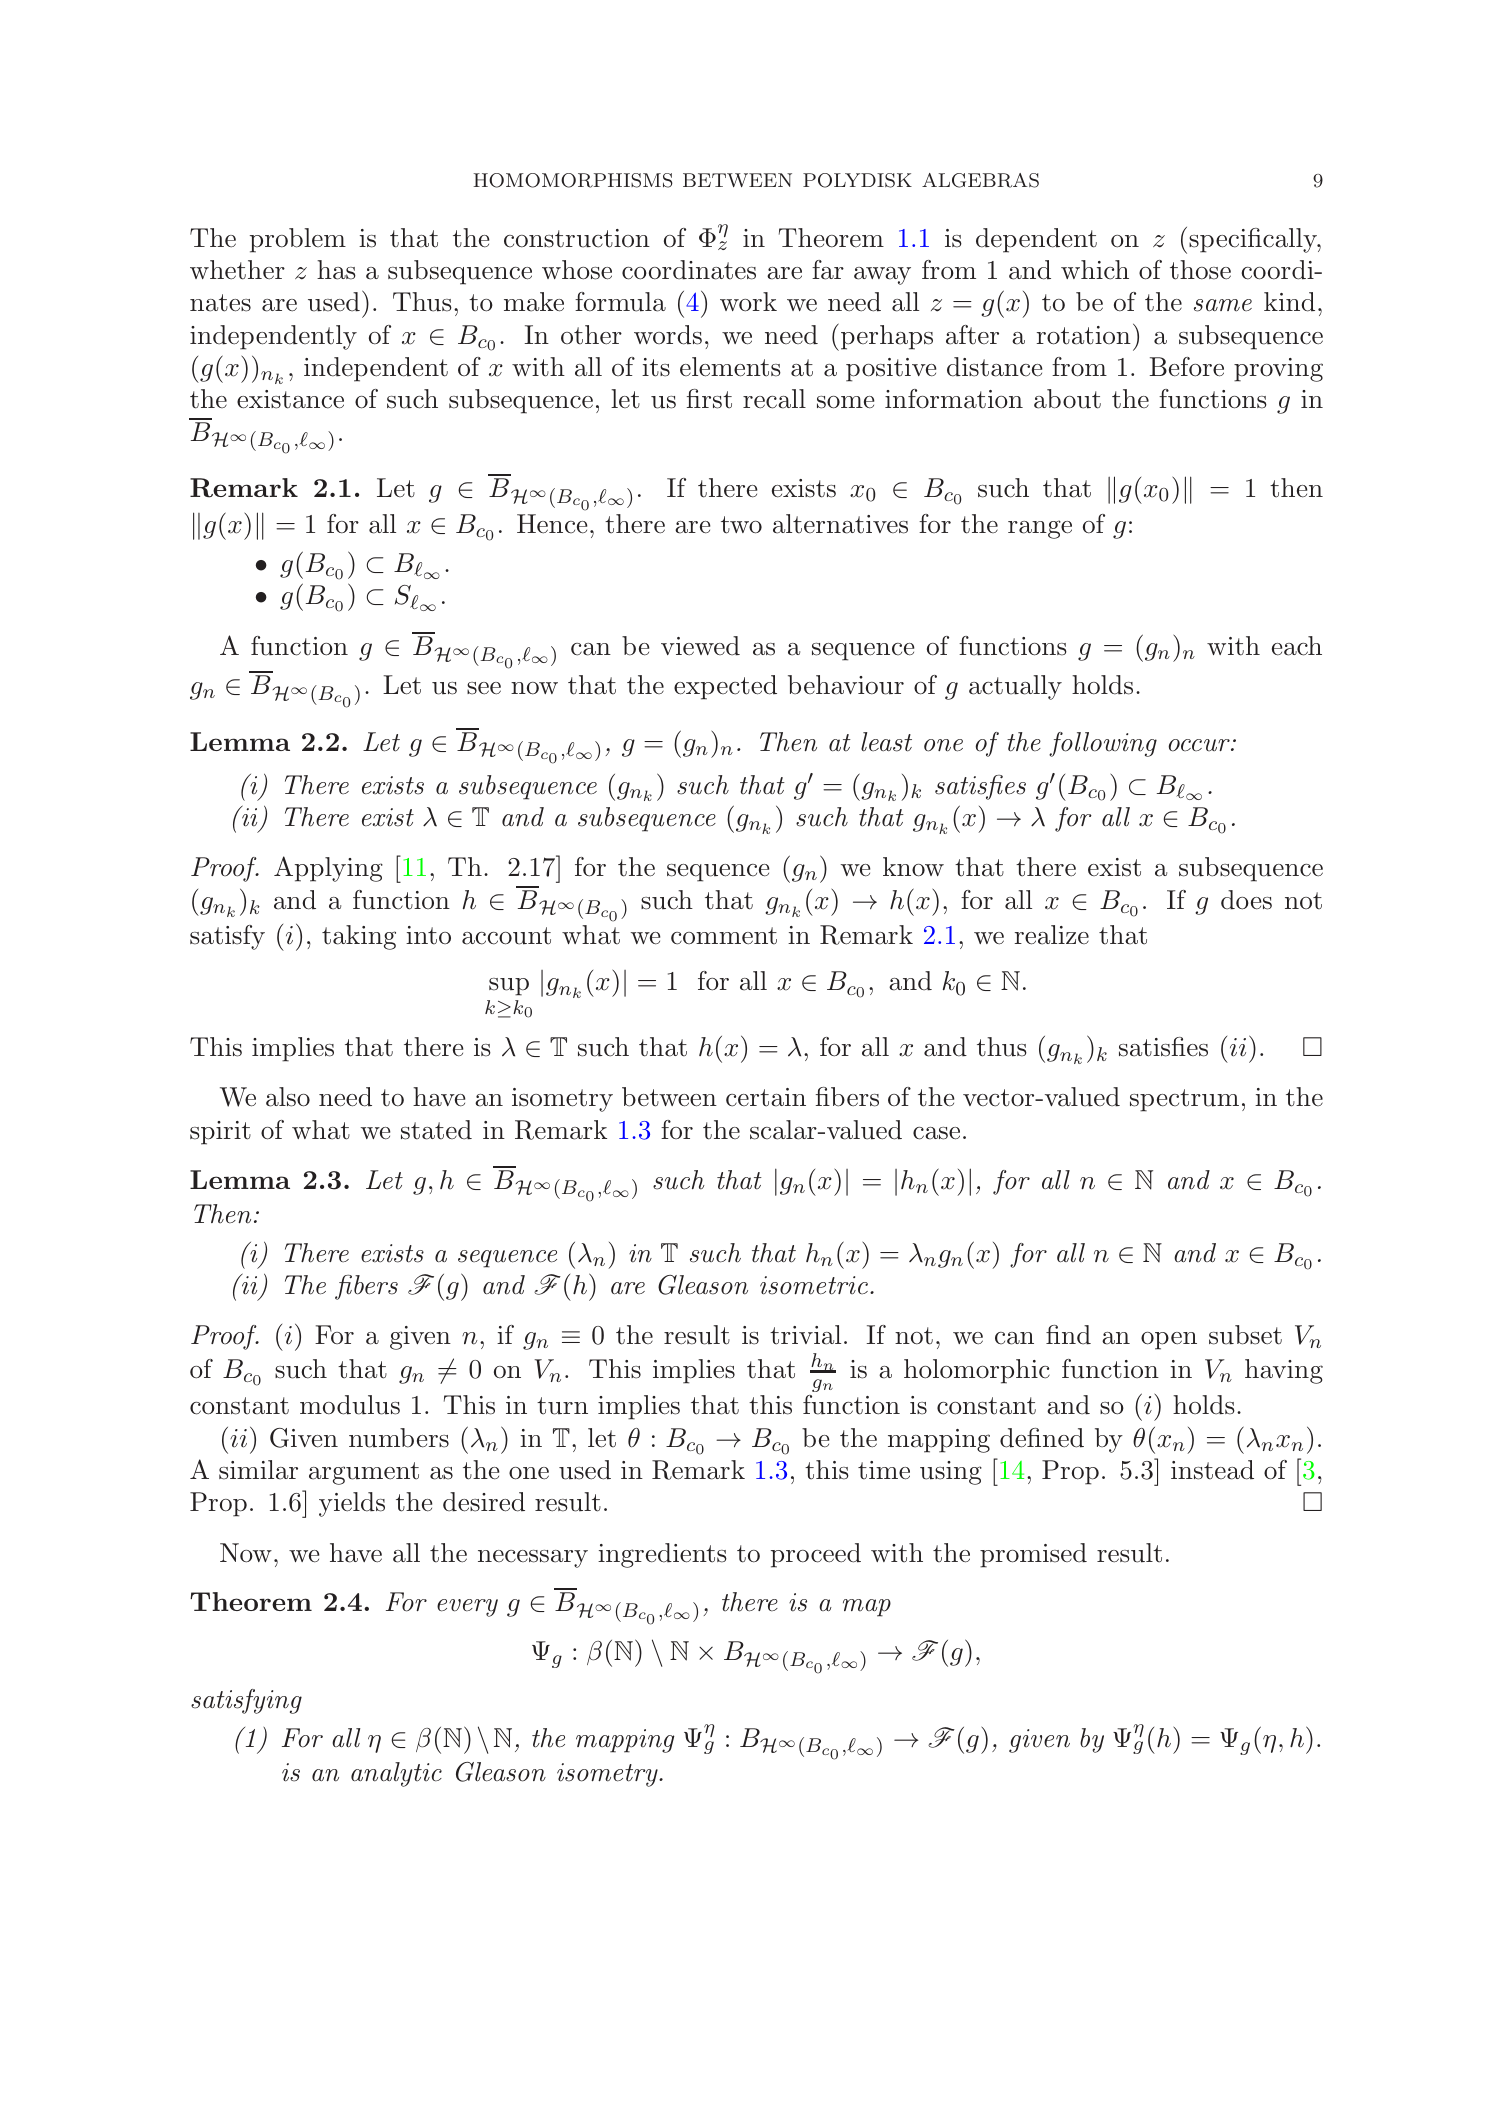
\includegraphics[width=0.90\textwidth]{figures/supporting_theorem_page9.png}
  \caption{The coordinate dichotomy and the start of Theorem 2.4.}
  \label{fig:support9}
\end{figure}

\begin{figure}[ht]
  \centering
  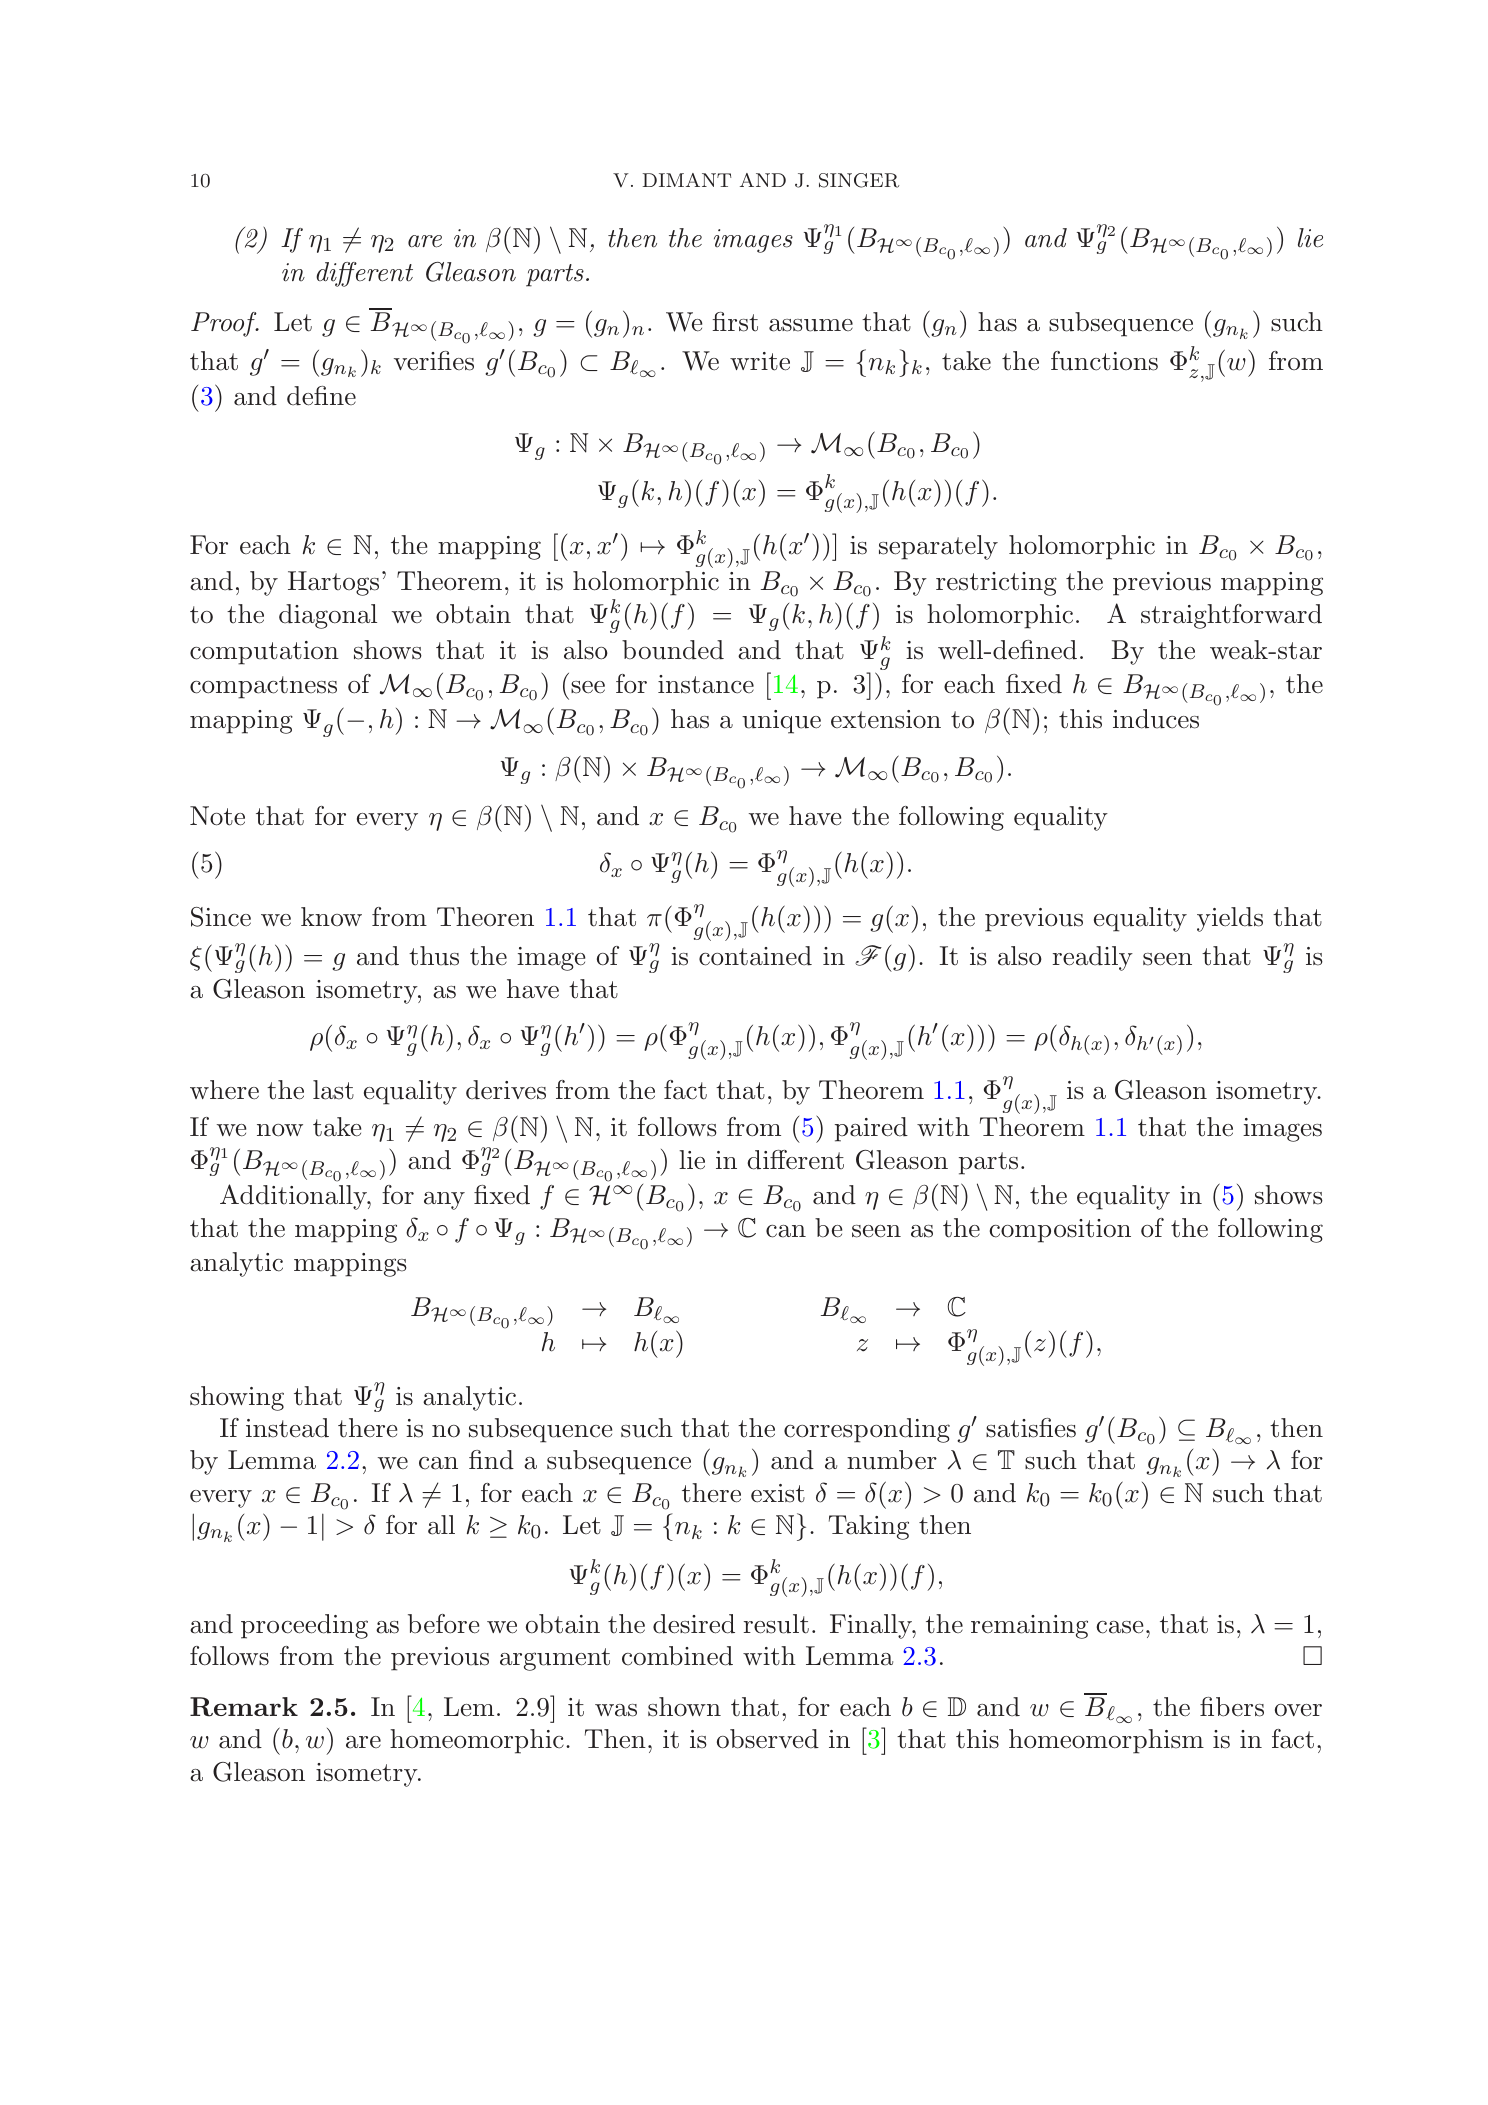
\includegraphics[width=0.90\textwidth]{figures/supporting_theorem_page10.png}
  \caption{The conclusion and proof of Theorem 2.4.}
  \label{fig:support10}
\end{figure}

\begin{thebibliography}{9}
\bibitem{DimantSingerFibered}
V. Dimant and J. Singer,
\emph{A fibered description of the vector-valued spectrum},
arXiv:1902.01387 (2019); Math. Nachr. 293 (2020), 2104--2124.

\bibitem{DimantSingerPolydisk}
V. Dimant and J. Singer,
\emph{Homomorphisms between algebras of holomorphic functions on the infinite
polydisk}, arXiv:1909.05105 (2019); J. Math. Anal. Appl. 489 (2020), 124131.
\end{thebibliography}

\end{document}
